\chapter{Implémentation De la méthode du Gap Statistique}

\startcontents[Implémentation]

\section{Implémentation De la méthode du Gap Statistique}

Dans cette partie, nous allons utiliser et comparer la performance du Gap Statistique aux autres méthodes. Nous allons dans un premier temps l'appliquer sur des données simulées et dans un second temps sur des données réelles.

\subsection{Cas des données simulées}
\subsection*{Données ayant un cluster}

\begin{figure}[H]
    \centering
    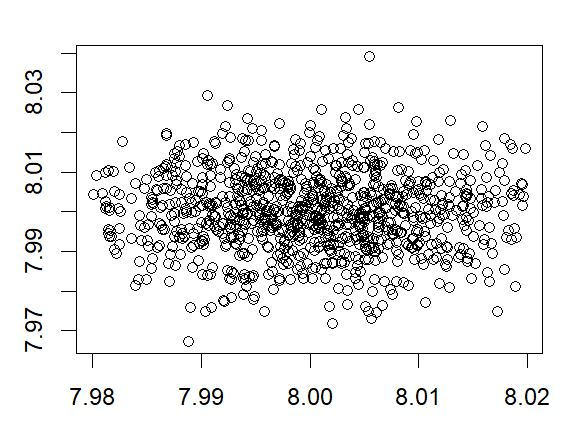
\includegraphics[width=0.5\linewidth]{images/don1.JPG}
    \caption{}
    \label{fig:enter-label}
\end{figure}

On constate que nos données n'ont pas de structure spécifique et semblent ne former qu'un seul groupe. 

La méthode de Kaufman et Rousseeuw (1990) identifie 7 clusters, ce qui, compte tenu des données, semble incohérent. Ce résultat est en accord avec la théorie exposée précédemment, car cette méthode n'est pas adaptée à des situations où un seul cluster est attendu. 
\subsection*{Méthode du Gap Statistique}

\begin{figure}[H]
    \centering
    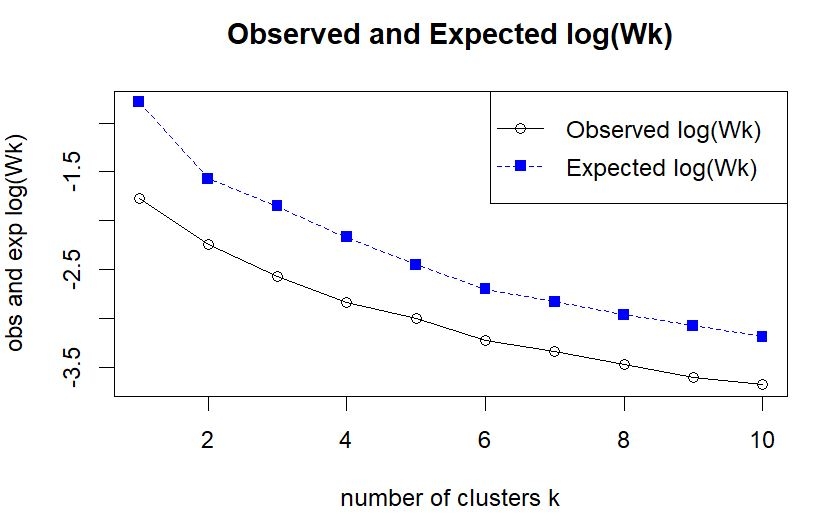
\includegraphics[width=0.5\linewidth]{images/Exp.JPG}
    \caption{}
    \label{fig:enter-label}
\end{figure}

On Constate en essayant d'observer la courbe du \(log(W_k)\) que la méthode du coude ne nous permet pas de conclure sur le nombre optimal de cluster. 

\begin{figure}[H]
    \centering
    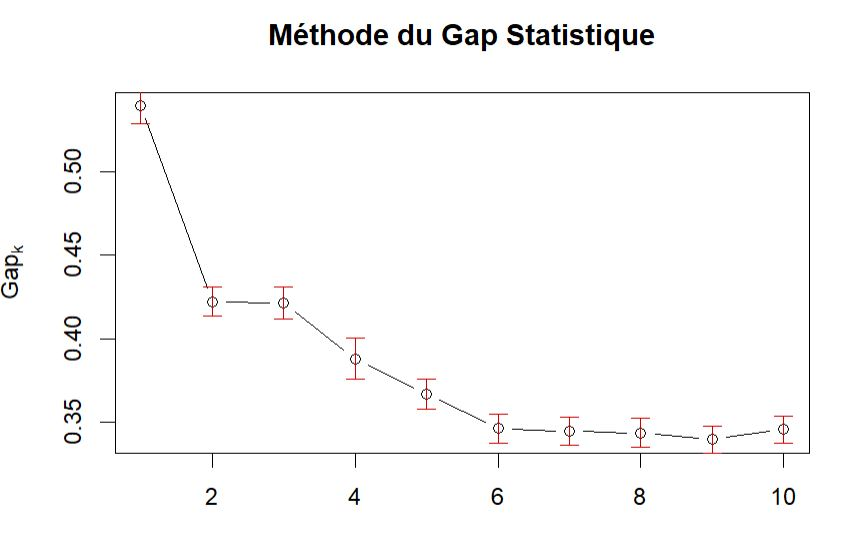
\includegraphics[width=0.5\linewidth]{images/Gaps.JPG}
    \caption{}
    \label{fig:enter-label}
\end{figure}


On constate que la méthode du Gap Statistique permet de donner de meilleurs résultats. En effet elle permet de conclure qu'il y a un seul cluster dans les données. ce qui correspond à la structure des données simulées. 

\newpage
\subsection{Données ayant trois clusters}
 Considérons maintenant un jeux de données simulé de façons à obtenir trois clusters et essayons de vérifier si la méthode du Gap Statistique permettra de trouver le même nombre de clusters.

\begin{figure}[H]
    \centering
    % 上面的大图
    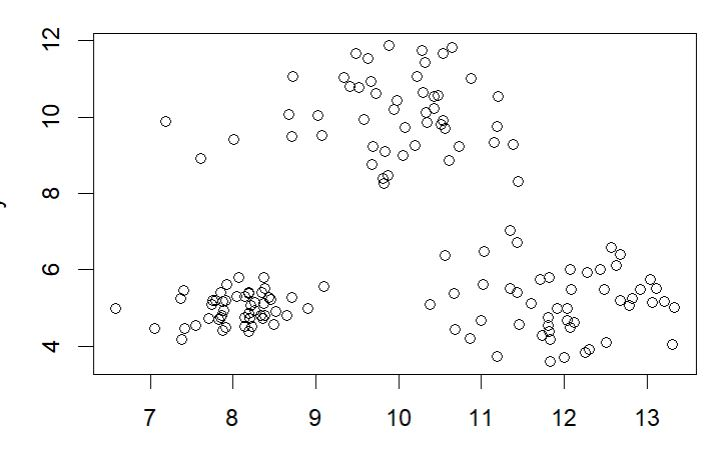
\includegraphics[width=0.7\linewidth]{images/obs2.JPG}
    \caption{}
    \label{fig:large-image}
    
    % 下面两个小图并排
    \begin{subfigure}[b]{0.45\linewidth} % 左侧子图
        \centering
        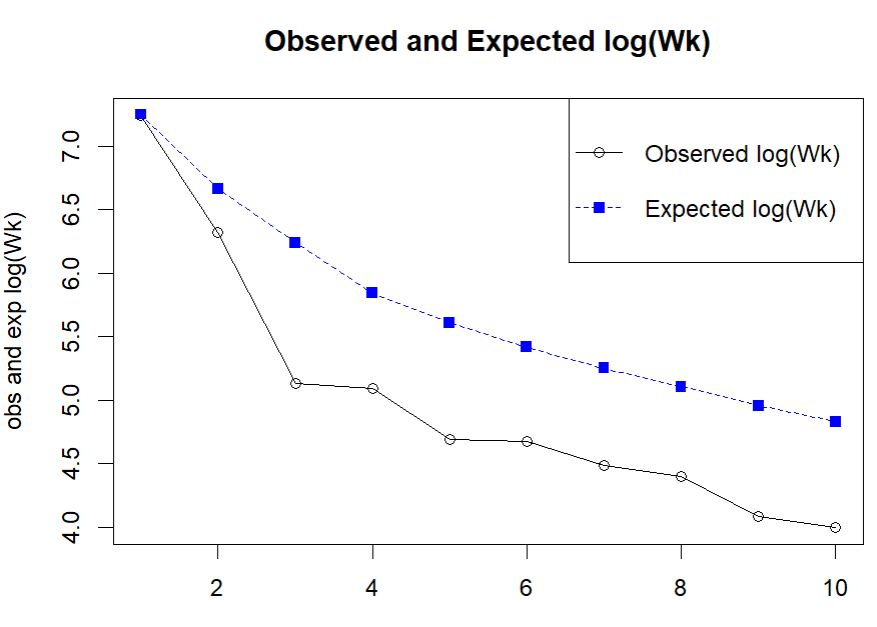
\includegraphics[width=\linewidth]{images/Exp2.JPG}
        \caption{Obs et Expected}
        \label{fig:Obs et Expected}
    \end{subfigure}
    \hspace{0.05\linewidth} % 两个子图之间的间距
    \begin{subfigure}[b]{0.47\linewidth} % 右侧子图
        \centering
        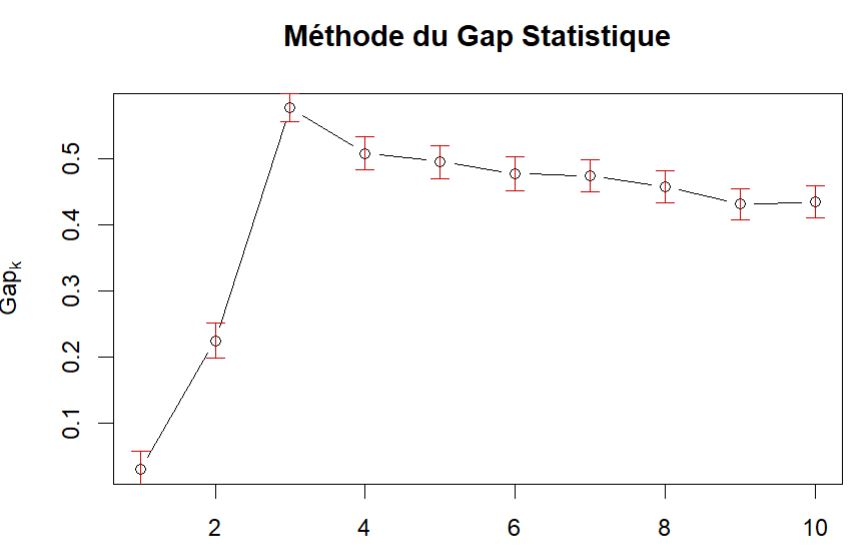
\includegraphics[width=\linewidth]{images/Gaps2.JPG}
        \caption{Gap statistique}
        \label{fig:right-small}
    \end{subfigure}
    \caption{}
    \label{fig:combined-figure}
\end{figure}

A l'aide de la règle du coude, on peut déduire que nous avons trois clusters dans notre jeux de données. De mémé, la méthode du Gap Statistique donnée par la figure (6) permet d'aboutir au même résultat. 

\newpage
\subsection{Cas d'une base de donnée réelle}

Nous allons dans cette sous section utiliser une base de données réelle. Nous avons choisis la base de données \textit{'Live'} qui contient des informations collectées auprès de vendeurs sur Facebook en Thaïlande. Les variables sélectionnées après avoir vérifié les éventuelles corrélations sont: (Le nombre total de commentaires sur la publication,Le nombre total de partages,Le nombre total de Like,Le nombre total de "Love",Le nombre total de "Wow","Haha" et de "Haha" )

En utilisant la règle du coude, on constate que le nombre de cluster optimal est entre 3 et 4 comme le montre la figure (7):

\begin{figure}[H]
    \centering
    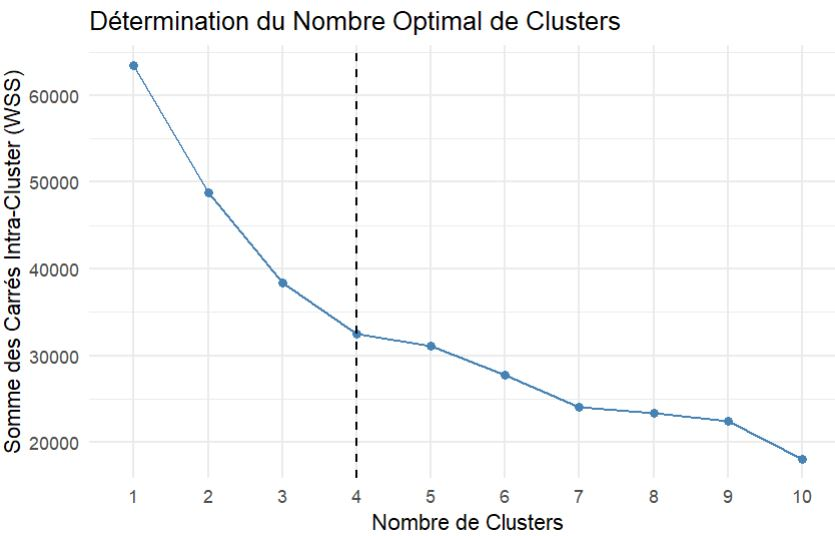
\includegraphics[width=0.8\linewidth]{images/Coude.JPG}
    \caption{}
    \label{fig:coude}
\end{figure}

En utilisant la méthode de Kaufman et Rousseeuw (1990) basée sur la statistique de la Silhouette, on obtient deux clusters avec un score optimal de 0.82.
 
En utilisant le Gap statistique, on obtient un seul cluster comme le montre la figure suivante. Ce qui semble ne pas être cohérent vu les résultats obtenus avec la méthode du coude. 

\begin{figure}[H]
    \centering
    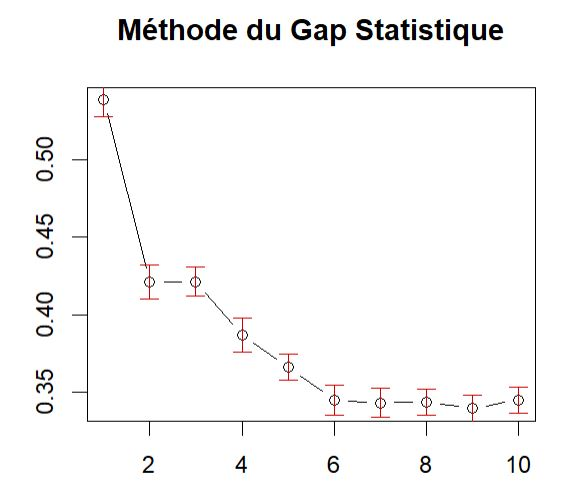
\includegraphics[width=0.6\linewidth]{images/Gap3.JPG}
    \caption{}
    \label{fig:gap3}
\end{figure}

Ce résultat, relativement imprécis, pourrait s'expliquer par deux facteurs principaux. D'une part, la méthode du Gap Statistique repose sur une hypothèse forte concernant la distribution des données, en supposant qu'elle suit une loi log-normale. D'autre part, la valeur espérée de \(log(W_k)\) est obtenue par des simulations numériques, ce qui la rend sensible au nombre de simulations effectuées ainsi qu'à la méthode employée pour générer ces données simulées.
